\section{Ombra Cornuta}\label{ombra-cornuta}

Tags: Personaggio Leggendario Creatore: Lorenzo Luogo: Foresta dei
Giganti

\section{Ombra Cornuta}\label{ombra-cornuta-1}

\begin{center}\rule{0.5\linewidth}{0.5pt}\end{center}

\begin{figure}
\centering
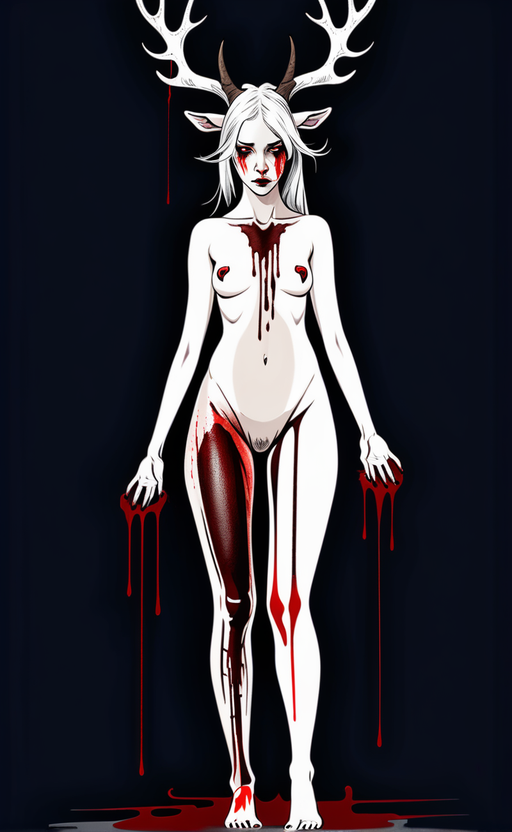
\includegraphics{young-woman-with-blood-on-her-skin-she-is-naked-has-legs-like-a-goat-and-horns-like-an-elk_(1).png}
\caption{young-woman-with-blood-on-her-skin-she-is-naked-has-legs-like-a-goat-and-horns-like-an-elk
(1).png}
\end{figure}

Informazioni Generali

Età: Sconosciuta

Data di nascita: Sconosciuta

Luogo di nascita: Foresta dei Giganti

Razza: Sconosciuta

Classe: Sconosciuta

Alleati:

Nemesi:

Alias:

Professione:

\begin{center}\rule{0.5\linewidth}{0.5pt}\end{center}

\subsection{1. Descrizione Generale}\label{descrizione-generale}

\begin{center}\rule{0.5\linewidth}{0.5pt}\end{center}

\begin{figure}
\centering
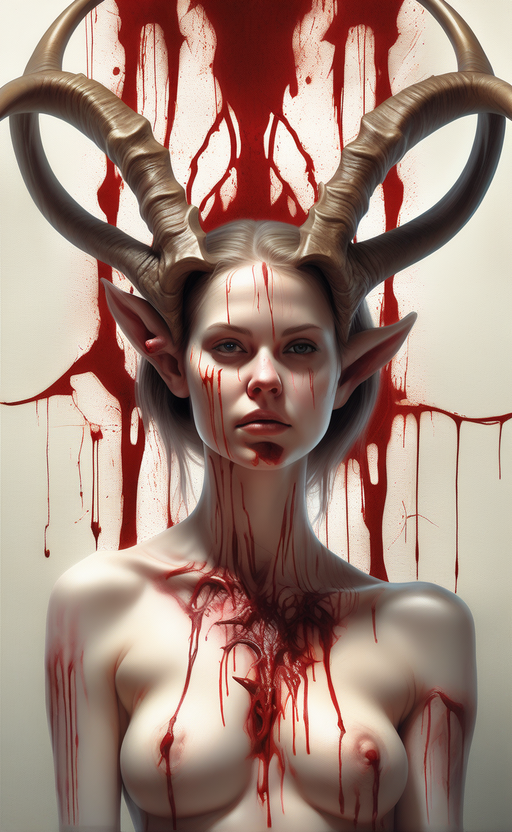
\includegraphics{young-woman-with-blood-on-her-skin-she-is-naked-has-legs-like-a-goat-and-horns-like-an-elk-sf-in.png}
\caption{young-woman-with-blood-on-her-skin-she-is-naked-has-legs-like-a-goat-and-horns-like-an-elk-sf-in.png}
\end{figure}

Nella misteriosa
\href{Foresta\%20dei\%20Giganti\%2003a15f8accd74ec0a08db3f3c9a26b2b.md}{Foresta
dei Giganti} si cela una presenza sfuggevole, un'entità che raramente si
manifesta agli sconsiderati che viaggiano attraverso la foresta,
un'ombra che vigila e che osserva. È conosciuta con molti nomi, la
Signora della Foresta, lo Spirito dei Giganti, la Dama nell'Ombra, ma è
conosciuta ai più come Ombra Cornuta.

Il suo aspetto sfugge alle descrizioni precise, nessuno conosce la vera
natura di questo essere. molti affermano di aver visto una donna con
grandi e possenti corna sul capo, con gambe e orecchie di capra, il cui
corpo nudo è coperto solo dal sangue; secondo altri invece si tratta di
un demonio assomigliante ad una capra antropomorfa, che cela il suo
aspetto con quello di una dolce fanciulla per attirare i mal capitati e
divorarli. Si dice che l'Ombra Cornuta sia lo spirito della foresta
stessa, rivelando la sua presenza solo a coloro che osano intraprendere
un viaggio attraverso gli alberi maestosi. Altri, invece, la temono come
un demone notturno che emerge solo per nutrirsi, lasciando dietro di sé
un alone di terrore e morte. Spirito benigno o demone malevolo che sia,
l'Ombra Cornuta vive tra leggenda e realtà, e le storie sul suo conto
spesso affolano le locande e i pensieri degli avventurieri.

\subsection{2. Storie}\label{storie}

\begin{center}\rule{0.5\linewidth}{0.5pt}\end{center}

Le leggende che circondano l'Ombra Cornuta sono numerose, e spaziano da
racconti avvincenti che ritraggono lo spirito come un'entità benevola, a
racconti che terrorizzano chiunque ascolti. Di seguito le leggende più
conosciute.

\subsubsection{2.1 Il commerciante
smarrito}\label{il-commerciante-smarrito}

C'era una volta un tessitore di stoffe proveniente dalla città di Kos,
che un giorno ricevette un ordine straordinario dal lontano villaggio di
Aihel. La richiesta era di una quantità enorme di tessuti, ma il
compratore chiedeva di recapitare l'intera merce entro soli 3 giorni. Il
povero tessitore sapeva bene che la strada per Aihel era lunga,
specialmente perché si allargava per evitare di passare attraverso la
foresta selvaggia.

Il coraggioso commerciante, tuttavia, non poteva permettersi di perdere
un ordine così importante. Così, nonostante la sua preoccupazione,
decise di rischiare e tagliare diritto attraverso la gigantesca foresta.
Era consapevole delle storie spaventose riguardo all'Ombra Cornuta, un
demone dall'aspetto femminile con gambe caprine e corna di cervo, temuto
da tutti gli abitanti della Foresta dei Giganti. Ma il dovere chiamava,
e il tessitore era determinato a portare a termine il suo compito.

Caricò il suo carretto con tutte le stoffe, legò il carretto al suo
fedele mulo e si avventurò nella foresta. Ben presto, però, calò la
notte, e il commerciante si perse tra gli alberi intricati e le ombre
inquietanti del bosco. La paura lo abbracciò, ma proprio quando sembrava
che la speranza lo abbandonasse, apparve l'Ombra Cornuta.

Il tessitore tremava di terrore di fronte a questa figura femminile
sporca di sangue, con corna maestose e occhi neri e lucenti. ``Il demone
mi ha trovato'', pensò con sgomento, ``ho osato sfidare la foresta e ora
riceverò la mia giusta punizione.'' L'Ombra Cornuta lo fissò per qualche
minuto, immobile davanti al dispero, poi si voltò e si mise a camminare
tra gli alberi.

Il tessitore, confuso e spaventato, senza sapere il motivo, decise di
seguire il demone attraverso i boschi. Quando l'Ombra Cornuta scomparve
alla vista, il tessitore continuò a seguire l'ombra proiettata dalle
maestose corna, illuminata dalla luce della luna. Per ore camminò, fino
a quando persino l'ombra svanì.

All'improvviso, si fermò, temendo di essere in guai ancora più grandi.
Ma alzando lo sguardo, notò delle luci lontane. Avvicinandosi, si rese
conto di essere giunto in un piccolo villaggio al di fuori della foresta
selvaggia.Il villaggio di Ahiel era ancora lontano, ma il tessitore,
grazie all'incontro con l'Ombra Cornuta, era riuscito a uscire dalla
foresta.

\subsubsection{2.2}\label{section}

\begin{center}\rule{0.5\linewidth}{0.5pt}\end{center}

Nella Foresta dei Giganti, dove gli alberi custodivano segreti antichi e
i boscaioli intrecciavano le loro vite con la natura, viveva un uomo di
nome Luk. Un giorno, mentre affilava la sua ascia per tagliare legna,
un'insolita visione catturò la sua attenzione: tra gli alberi più
lontani, danzava una giovane fanciulla, vestita solo dalla nudità della
sua innocenza.

Luk, colto dall'emozione e dalla sorpresa, corse immediatamente dai suoi
colleghi per condividere la straordinaria visione. I suoi compagni
boscaioli credettero alla sua storia e si precipitarono tra gli alberi
per cercare la misteriosa fanciulla. Tuttavia, nonostante la loro
ricerca instancabile, la giovane scomparve come un sogno sfuggente.

I boscaioli, delusi, si rivoltarono contro Luk, accusandolo di inganni e
menzogne. Il giorno successivo, però, la fanciulla si materializzò
nuovamente tra gli alberi, confermando la veridicità delle parole di
Luk. Nonostante ciò, il suo racconto fu nuovamente accolto con
scetticismo, e la comunità lo derise come un fabulatore.

Determinato a dimostrare la sua verità, Luk decise di affrontare la
situazione da solo. Nel terzo giorno, quando la fanciulla si ripresentò,
Luk, armato di ascia, decise di seguirla da solo. Questa volta, non
permise che la sua preda sfuggisse tra le ombre degli alberi.

Man mano che la foresta si faceva sempre più densa, il panico si insinuò
nel cuore di Luk. Si ritrovò nel bel mezzo della foresta selvaggia,
incapace di rintracciare la via di casa. Proprio quando la disperazione
cominciava a stringerlo, la fanciulla con le corna e gli artigli si
palesò davanti a lui.

Con una freddezza spaventosa, la creatura gli svelò la sua vera natura.
Luk, terrorizzato, venne brutalmente ucciso e il demone si cibò del suo
corpo senza pietà. Da quel giorno, la storia di Luk e della sua inusuale
scoperta divenne una leggenda, un monito per coloro che osavano sfidare
i misteri delle foreste oscure.

\subsection{3. Coinvolgimenti in Eventi
Recenti}\label{coinvolgimenti-in-eventi-recenti}

\begin{center}\rule{0.5\linewidth}{0.5pt}\end{center}

\href{Untitled\%20Database\%20f4f70c0cf72f46ecb12f8c8b3a15302c.csv}{Untitled
Database}

\subsection{A. Scheda Personaggio}\label{a.-scheda-personaggio}

\begin{center}\rule{0.5\linewidth}{0.5pt}\end{center}

\href{Info\%20PG\%20671ef2a33d454743bb2b7f3bb59c3144.csv}{Info PG}

\subsubsection{Statistiche e abilità}\label{statistiche-e-abilituxe0}

\begin{center}\rule{0.5\linewidth}{0.5pt}\end{center}

\href{Abilita\%CC\%80\%2047ae4f9c53dd4179b08562154b33a396.csv}{Abilità}

\subsubsection{Lista magie}\label{lista-magie}

\subsection{B. Galleria Immagini}\label{b.-galleria-immagini}

\begin{figure}
\centering
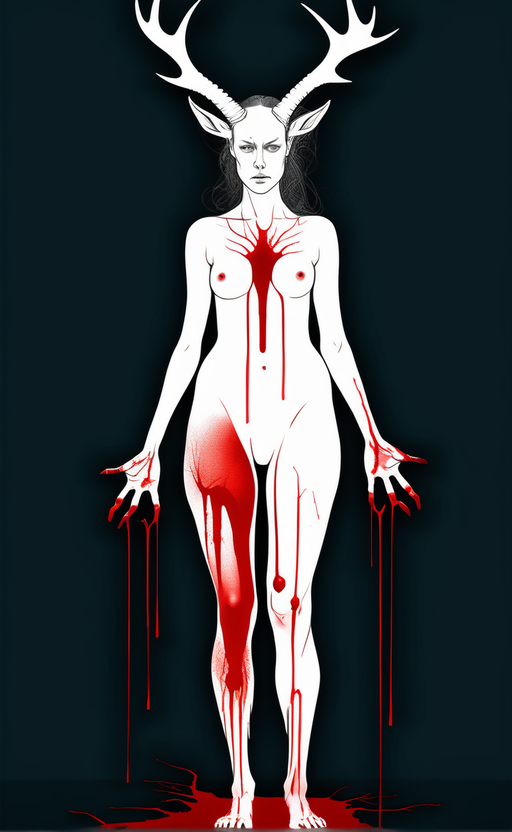
\includegraphics{young-woman-with-blood-on-her-skin-she-is-naked-has-legs-like-a-goat-and-horns-like-an-elk-sf-in_(1).png}
\caption{La maggior parte delle sue raffigurazione sui libri dedicati
alle leggende della Foresta dei Giganti la ritraggo come una donna
sporca di sangue e con delle ampie corne simili a quelle di un cervo.
Spesso non è fatto alcun cenno ai piedi da capra.}
\end{figure}

La maggior parte delle sue raffigurazione sui libri dedicati alle
leggende della Foresta dei Giganti la ritraggo come una donna sporca di
sangue e con delle ampie corne simili a quelle di un cervo. Spesso non è
fatto alcun cenno ai piedi da capra.

\begin{figure}
\centering
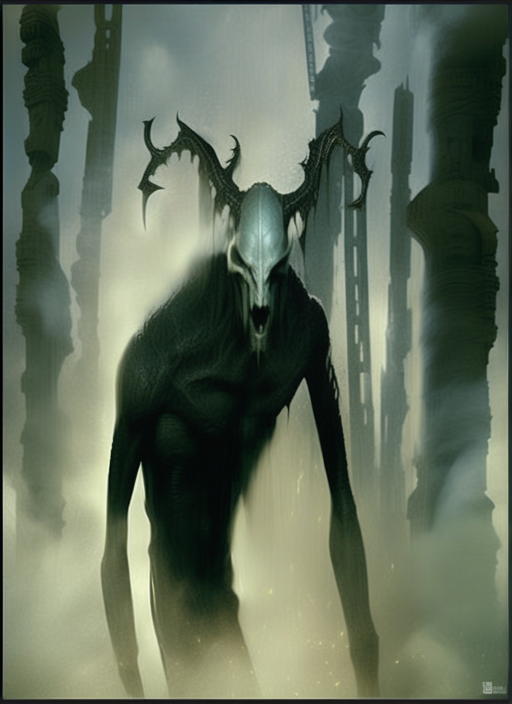
\includegraphics{demon-sf-intricate-artwork-masterpiece-ominous-matte-painting-movie-poster-golden-ratio-trendi.png}
\caption{Una credenza comune vuole che l'Ombra Cornuta non sia altro che
un demone attira le sue prede mutando il suo aspetto in quello di una
donna.}
\end{figure}

Una credenza comune vuole che l'Ombra Cornuta non sia altro che un
demone attira le sue prede mutando il suo aspetto in quello di una
donna.

\subsection{A. Descrizione Originale}\label{a.-descrizione-originale}

\begin{center}\rule{0.5\linewidth}{0.5pt}\end{center}
